\subsection{Об алгоритмах и программах. Программные реализации.}
\label{sec:2a}

Реализацию экспериментального программного обеспечения можно разделить
на три части:

\begin{itemize}
\item{Реализация метода молекулярной динамики}
\item{Реализация генетического алгоритма}
\item{Реализация подсистемы для решения задачи нахождения равновесной конфигурации
двумя перечисленными способами и сравнения их эффективности}
\end{itemize}

Схема взаимодействия перечисленных подсистем изображена на рис.~ \ref{system_implementation}

\begin{figure}[ht!]
 \begin{center}
 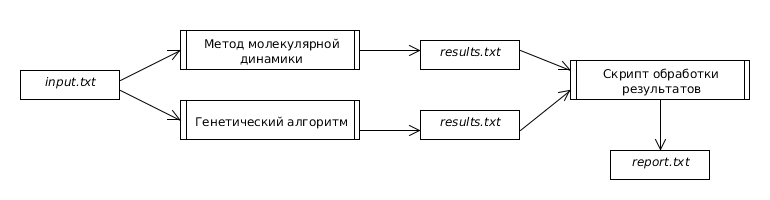
\includegraphics[width=0.9\textwidth]{FIGs/system_implementation.png}
 \end{center}
 \caption {Схема взаимодействия компонентов разработанного ПО}
 \label{system_implementation} 
\end{figure}

Метод молекулярной динамики и генетический алгоритм реализованы в качестве
отдельных приложений, не взаимодействующих друг с другом напрямую. Запуск этих
приложений и анализ результатов их выполнения реализован с помощью управляющего скрипта
командной оболочки Bash. В качестве интерфейса между управляющим скриптом и
приложениями, находящими равновесную конфигурацию, выбран интерфейс текстовых файлов.
Такой подход позволяет сделать всю систему модульной, где каждый компонент легко
заменяем. Так как непосредственно вычисления равновесной конфигурации занимают значительно
больше процессорного времени, чем чтение и запись текстовых данных на диск, то
выбор текстовых файлов в качестве интерфейса является уместным.

Входными данными для приложений является начальная пространственная конфигурация нанокластера,
представляющая собой матрицу из $N \times 3$ элементов. Для её представления выбран формат
.mat, использующийся для выгрузки и загрузки различных математических объектов в таких
математических пакетах как Matlab и Octave. Формат .mat представляет из себя простой текстовый
файл, где хранятся данные о структуре и значениях математического объекта. В рамках данной работы
был реализован парсер этого формата в виде библиотеки на языке С, что позволило подключить
его к обоим разработанным приложениям.

Метод молекулярной динамики реализован на языке Fortran-90 и не использует сторонних математических
библиотек. Блок-схема программы представлена на рис. \ref{block_MD}

\begin{figure}[ht!]
 \begin{center}
 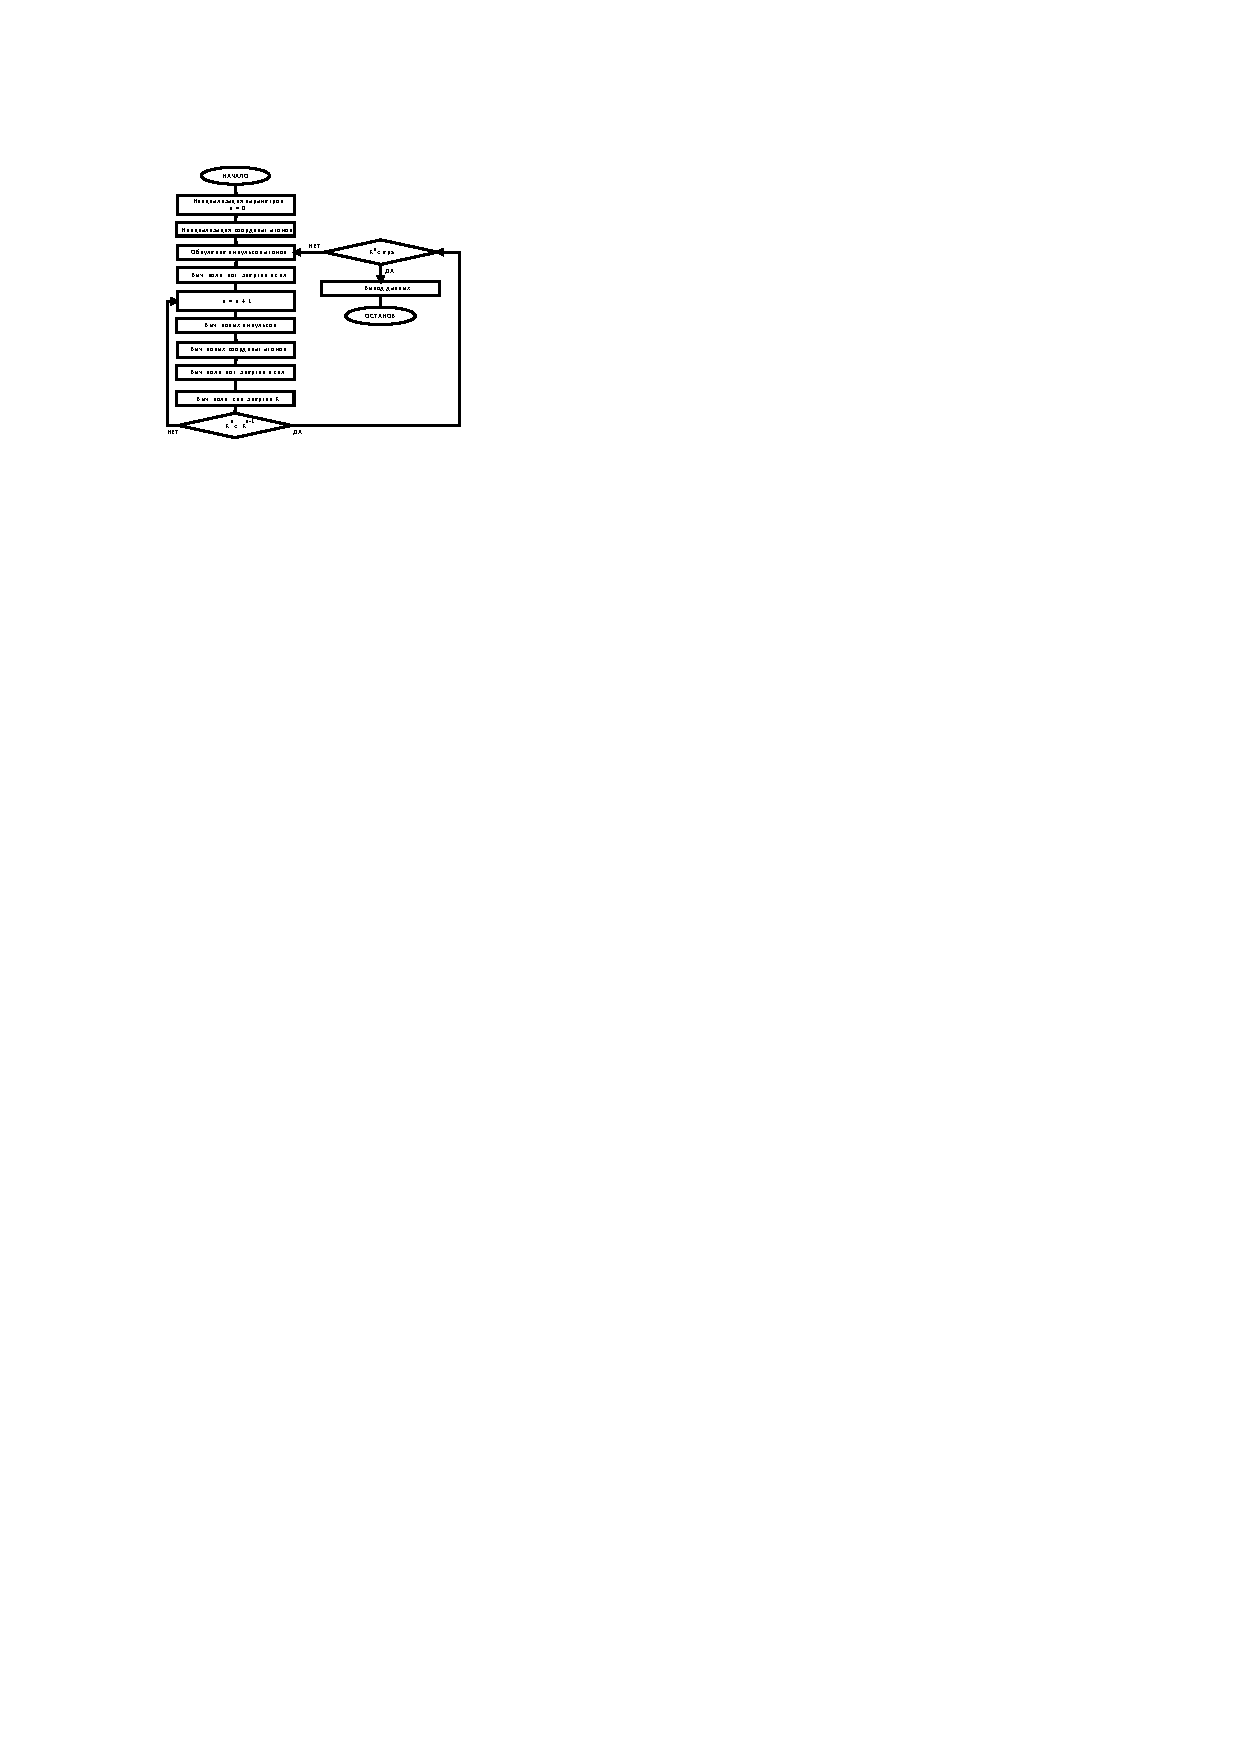
\includegraphics[width=0.9\textwidth]{FIGs/MD1crop.pdf}
 \end{center}
 \caption {Блок-схема реализации метода молекулярной динамики}
 \label{block_MD} 
\end{figure}

